\documentclass[a4paper,11pt]{article}
\usepackage{graphicx}
\usepackage[utf8]{inputenc}
\usepackage[activeacute,spanish]{babel}

\title{Manual Sudoku 0.3}
\author{Iván Aveiga \\ Kevin Campuzano}

\begin{document}

\maketitle


\newpage

\section{Información}
	Sudoku es un juego en donde en una cuadrícula de 9x9 no debe de tener números repetidos en filas, columnas o subcuadrícula de 3x3.
	
	\begin{center}
		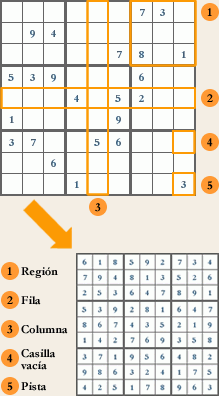
\includegraphics[width = 0.4\textwidth]{reglas.png} \footnote{http://www.sudokumania.com.ar/sm1/images3/reglas.png}
	\end{center}

\section{Aspectos Técnicos}
	Implementamos un juego de Sudoku en que el usuario debe resolver un tablero de sudoku según la difucultad elegida, entre estas tenemos.
	\begin{itemize}
		\item Fácil: 36-41 casillas llenas.
		\item Normal: 32-35 casillas llenas.
		\item Avanzado: 28-31 casillas llenas.
		\item Experto: 23-27 casillas llenas.
	\end{itemize}
	 
	 \subsection{Algoritmo}
	 	Se carga internamente un sudoku aleatoriamente entre cuatros sudokus almacenados en texto plano, dependiendo de la dificultad se seleccionan casillas aleatoriamente para usar en el tablero en que el usuario jugara. Se usa el concepto de random walks, para la selección de casillas se usó Programming Sudoku [Wei Meng].
		El usuario puede verificar si las casillas estan correctamente colocadas dando clic en el botón verificar.
	\subsection{Interfaz Gráfica}
		Al iniciar la aplicación se muestra una ventana donde ingresar el nombre y la dificultad a jugar.
		\begin{center}
		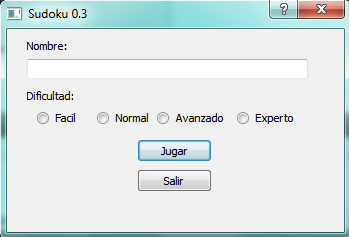
\includegraphics[width=0.5\textwidth]{inicio.png}
		\end{center}
		
		Una vez ingresado el nombre y seleccionada la dificultad aparece la ventana a jugar, mostrada a continuación.
		\begin{center}
			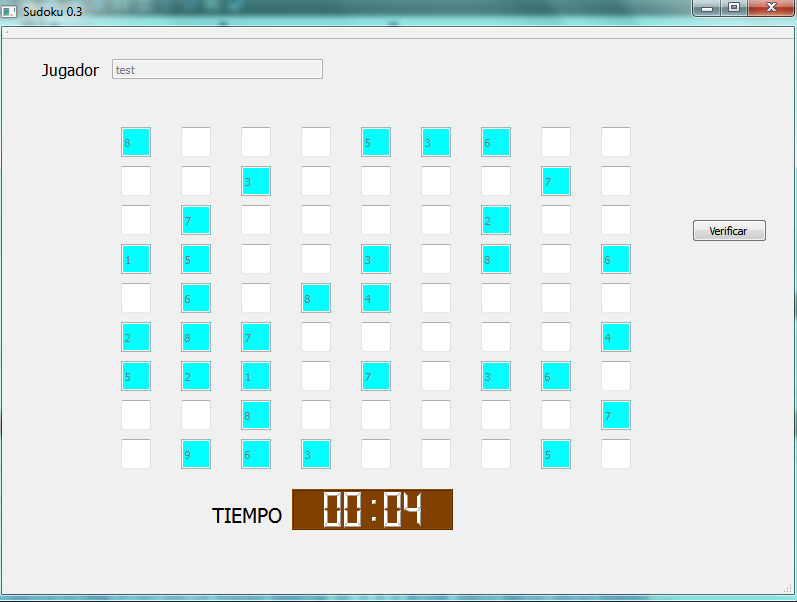
\includegraphics[width = 0.6\textwidth]{juego1.png}
		\end{center}
	 
	 Podemos ver el ingreso de números validados a un solo dígito y que por motivos de ilustración podemos ver que las celdas erróneas luego de dar clic en el botón verificar se tornan de color magenta.
	 
	 \begin{center}
	 	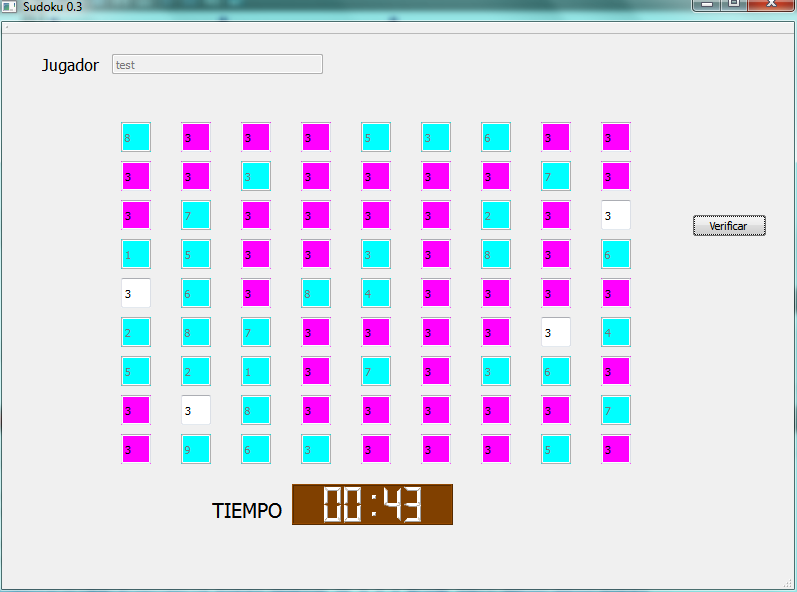
\includegraphics[width = 0.5\textwidth]{juego2.png}
	 \end{center}
	 
	 Al resolver correctamente el tablero el cronómetro se paraliza y se muestra el mensaje de que el usuario ganó.
	 \begin{center}
	 	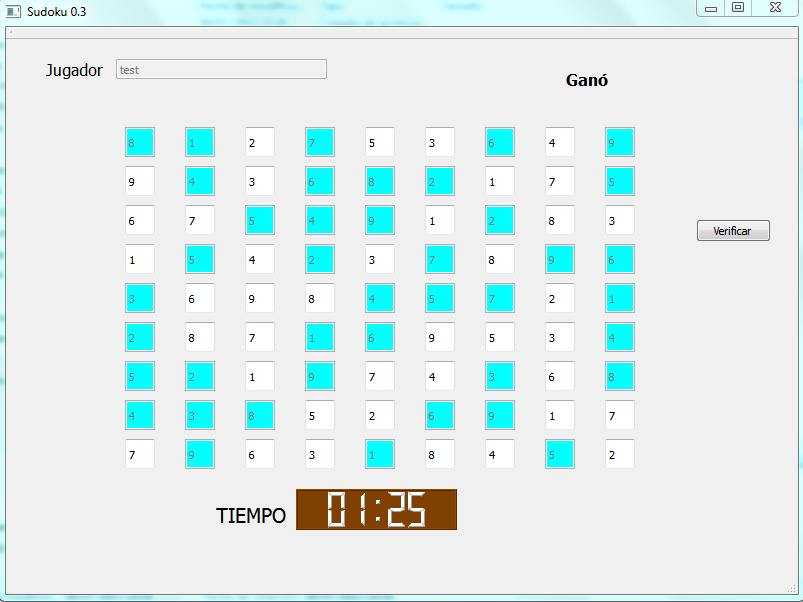
\includegraphics[width = 0.5\textwidth]{juego3.png}
	 \end{center}
	 
	 
\end{document}
